\section{Metaheurística GRASP}
\subsection{Descripción del algoritmo}
Una heuristica GRASP es un proceso iterativo, en el cual cada iteración consiste en dos fases, una constructiva, en la cual una posible solución es producida y otra fase con una busqueda local en la cual se encuentra un óptimo local en una vecindad definida por la solución construida en la primera fase.
La mejor solución obtenida se devuelve como resultado.
El siguiente pseudocodigo describe el procedimiento de GRASP.

\subsubsection{Pseudocódigo de GRASP}
\begin{algorithm}[H]
\begin{algorithmic}[1]
\caption{GRASP(Grafo G, Nat k, Nat maxIter)}
\STATE mejorSolucion $\leftarrow$ $\infty$
\WHILE {criterioDeParada(maxIter)}
    \STATE solucionGolosa $\leftarrow$ HeuristicaGolosaAleatorizada(G,k, etc.)
    \STATE solucionLocal $\leftarrow$ busquedaLocal(G,k,solucionGolosa,etc.)
    \IF{solucionLocal $<$ mejorSolucion}
        \STATE mejorSolucion $\leftarrow$ solucionLocal 
    \ENDIF
\ENDWHILE
\RETURN mejorSolucion
\end{algorithmic}
\end{algorithm}

\textit{criterioDeParada} es una función que devuelve cuando para el algoritmo. Las utilizamos para evitar que corra infinitamente y para garantizar una solución en tiempo razonable. 

Implementamos dos criterios:
\begin{enumerate}
    \item \textit{Cantidad Máxima de Iteraciones}: el ciclo termina cuando llega a hacer una prefijada cantidad de iteraciones 
    \item \textit{Iteraciones sin Mejora}: el ciclo termina cuando hace una prefijada cantidad de iteraciones sin mejorar la \textit{mejorSolucion} hasta el momento.
\end{enumerate} 
También se puede implementar una combinación de ambas, entonces el ciclo termina cuando ocurre alguna de las dos cosas. (estos criterios son analizados en mayor profundidad en la sección de \textit{Testing}).

GRASP También hace la función \textit{HeuristicaGolosaAleatorizada} para obtener una solución inicial para la posterior optimización de la busqueda local.
Esta es una modificación de la Heuristica Golosa presentada anteriormente, con ciertas decisiones aleatorizadas.

Presentamos el pseudocódigo de la misma:

\subsubsection{Pseudocódigo de la heurística golosa aleatorizada}
\begin{algorithm}[H]
\begin{algorithmic}[1]
\caption{HeuristicaGolosaAleatorizada(Grafo G, Nat k, Nat profundidadVertice, Nat profundidadConjunto)}
\STATE Vector$<$Conjunto$<$Nat$>>$ \textbf{conjuntos}(k, vacío)
\STATE Vector$<$Nat$>$ \textbf{nodosOrdenados} $\leftarrow$ OrdenarNodosPorPesoMayorAMenor(G)
\STATE Nat $cantidadConjuntosCandidatos$ $\leftarrow$ minimo(k, profundidadConjunto)
\WHILE {\NOT \textbf{nodosOrdenados}.vacio()}
    \STATE Nat $cantidadVerticesCandidatos$ $\leftarrow$ minimo(\textbf{nodosOrdenados}.size(), profundidadVertice)
    \STATE $verticeNuevo$ $\leftarrow$ Elegir de manera aleatoria un nodo de \textbf{nodosOrdenados} entre las primeras $cantidadVerticesCandidatos$ posiciones
    \STATE Borrar a $verticeNuevo$ de \textbf{nodosOrdenados}
    \STATE Ordenar \textbf{conjuntos} por el peso del $verticeNuevo$ en ellos de menor a mayor
    \STATE Elegir de manera aleatoria un $conjunto$ de \textbf{conjuntos} entre los primeras $cantidadConjuntosCandidatos$ posiciones
    \STATE Insertar $nuevoVertice$ en $conjunto$
\ENDWHILE
\RETURN conjuntos
\end{algorithmic}
\end{algorithm}

Los puntos claves del algoritmo anterior son en la randomización de elecciones:
\begin{enumerate}
    \item \textit{Profundidad de la elección de nodos}: el algoritmo goloso sin randomización ordena decrecientemente los nodos por peso y luego elige siempre el primero para colocarlo en algún subconjunto, pero aquí determinamos un entero $v$ que va a servir como parámetro para elegir aleatoriamente entre los $v$ primeros nodos.
    \item \textit{Profundidad de la elección de conjuntos}: en la versión sin aleatoriedad siempre se elige colocar el nodo en cuestión dentro del subconjunto en el cual tenga peso mínimo, en cambio en este se determina un entero $s$ que sirve como parámentro para elegir aleatoriamente entre los $s$ subconjuntos donde el nodo tenga el menor peso.
\end{enumerate} 
Ademas de que uno elige sobre nodos y el otro sobre conjuntos, la diferencia entre los dos puntos anteriores es que el orden del primer punto se determina al principio del algoritmo y no cambia a lo largo de la ejecución, a diferencia del segundo punto que su orden varia en tiempo de ejecución. Estos items son profundizados en la siguiente sección de \textit{testing}.


\subsection{Tests}
Mostraremos los resultados de varios tests realizados a la GRASP, los cuales introducimos brevemente:
\begin{itemize}
    \item \textbf{Test de configuración}: Dado un conjunto de instancias, busca la mejor configuración de la GRASP, variando criterios de parada y de selección de la lista de candidatos (RCL) de la heurística golosa aleatorizada.
    \item \textbf{Test de calidad}: Para un conjunto reducido de instancias, se compara cuánto más pesada es la solución de la GRASP en relación a la solución óptima, usando la configuración ganadora del test anterior.
    \item \textbf{Test de tiempo de ejecución}: Dado un conjunto de instancias, se calculan los tiempos de ejecución de la GRASP para distintas configuraciones.
\end{itemize}

El conjunto de instancias utilizado está compuesto por 100 instancias para cada \\ ${n = 3, ..., 100}$ y tiene las siguientes características:
\begin{enumerate}
    \item Los pesos de las aristas de los grafos pertenecen al intervalo cerrado $[\num{0.0001}, \num{1000}]$.
    \item Sea $G = (V,X)$ con $n = |V|$ y $m = |X|$ un grafo cualquiera del conjunto.\\ Sea $m_{max} = \frac{n(n-1)}{2}$. Entonces,
            \begin{align*}
                \num{0.7} \cdot m_{max} \leq m \leq m_{max} 
            \end{align*}
            Esto lo hicimos para evitar tener instancias con grafos fáciles de resolver incluso para la heurística golosa. Esto es claro en el caso extremo de que el grafo no tenga aristas. Teniendo esto en cuenta, pedimos que al menos tengan $70\%$ de la máxima cantidad de aristas posibles para cada grafo.
    \item Sea $G = (V,X)$ con $n = |V|$ un grafo cualquiera del conjunto. Entonces,
            \begin{align*}
                        2 \leq k \leq max\left(2, \frac{n}{3}\right)
            \end{align*}
            La razón de esto es la misma que en el punto anterior. En el caso extremo, si tuviéramos un grafo con $k \geq n$, alcanzaría con poner un vértice en cada conjunto para obtener una solución óptima (en el otro extremo, $k = 1$ sólo admite una solución, que obviamente es óptima). A mayor $k$, más márgen de error se le da a la heurística para equivocarse porque tiene más conjuntos donde colocar vértices. Por este motivo limitamos a $\frac{n}{3}$ la cantidad de conjuntos que puede tener una partición.
\end{enumerate}
Las instancias fueron generadas aleatorizando cada una de las variables mencionadas. El código del generador se encuentra en el Apéndice.


\subsubsection{Test de configuración}

Lo que primero necesitamos es tener una idea de cuál configuración usar en la GRASP. Para ello, testearemos con todas las combinaciones de configuraciones para un set acotado de valores, y discutiremos al respecto sobre cómo interpretar los resultados obtenidos, y así decidir una configuración.

Tenemos dos criterios de parada: parar por un límite $\alpha$ de iteraciones máximo, o parar si una cierta cantidad $\beta$ de instancias pasaron sin haber mejora en la solución. Por el el lado de la heurística aleatorizada, es decir, para la selección de candidatos, tenemos dos variables independientes: la profundidad de la elección del próximo vértice a insertar, y la profundidad de la elección del conjunto en que va a ser insertado el vértice.

Parar por un máximo de iteraciones $\alpha$ es el criterio más sencillo, pero tiene inconvenientes. Por un lado, podemos estar haciendo muchas iteraciones de más ya que rápidamente encontramos la solución óptima; esto ocurre siempre con grafos con pocos nodos, que son fáciles de resolver. Por otro lado, puede pasar que la cantidad fija de iteraciones que fue seteada no sea suficiente, y que obtengamos soluciones subóptimas incluso para lo que puede dar GRASP.

Parar por iteraciones sin mejora es más flexible porque si se encuentra rápidamente la solución óptima, no va a haber mejora en las próximas $\beta$ iteraciones, por lo cual el algoritmo va a terminar mucho más rápido para este tipo de casos. Para el caso en que sí haya mejoras todo el tiempo, incluso aunque $\beta < \alpha$ el algoritmo seguirá ejecutando hasta que pasen $\beta$ iteraciones sin mejorar, lo cual puede hacer que el total de iteraciones sea mucho mayor a $\alpha$, pero consiguiendo una solución con mejor calidad que parar por máximo de iteraciones. De todas formas, podría pasar que las soluciones obtenidas de la golosa y mejoradas con la búsqueda local, sean peores que la mejor hasta el momento durante $\beta$ iteraciones, y que si $\beta < \alpha$, se termine haciendo menos iteraciones que $\alpha$, por lo cual no hay garantía de que parar por iteraciones sin mejora en el caso $\beta < \alpha$ vaya a devolver mejores soluciones que parar en $\alpha$ iteraciones.

Si tomamos $\beta < \alpha$, cabe preguntarse qué valor de $\beta$ hace falta para que parar por iteraciones sin mejora sea mejor que parar por máximo de iteraciones. Fijamos $\alpha = 100$, y testeamos con $\beta = 10, 35, 50, 70$.

Pero todavía falta la selección de candidatos: plantearemos que ambas profundidades puedan tomar los valores $1$, $2$ ó $4$. Como notación, cuando decimos \underline{profundidad $(x_1,x_2)$} significa profundidad de elección de vértice $x_1$ y profundidad de elección de conjunto $x_2$. Notar que la profundidad $(1,1)$ es equivalente a la golosa pura, sin aleatoriedad. Dejamos esa opción para verificar que la aleatoriedad es efectivamente necesaria para obtener mejores soluciones. Con respecto a esto, conjeturamos que lo mejor es aleatorizar lo máximo posible, entonces esperamos ver que $(4,4)$ sea la mejor configuración de selección.

Dado un $n$, para cada instancia que tenga un grafo de $n$ nodos, se va ejecutar GRASP con cada configuración por separado y se van a acumular los resultados. Luego, se busca cuál es la mejor configuración para este $n$ hallando el mínimo de las sumas de pesos para cada configuración. El mínimo se calcula de la siguiente manera:
\begin{algorithm}[H]
\begin{algorithmic}[1]
\caption{Cálculo del mínimo peso de las configuraciones para un $n$}
\STATE mejorPesoAcumulado $\leftarrow$ $+ \infty$
\FOR {valor de iteraciones sin mejora (10, 35, 50, 70)}
    \FOR{cada valor de profundidad de vértice (4, 2, 1)}
        \FOR{cada valor de profundidad de conjunto (4, 2, 1)}
            \IF{Peso acumulado de esta configuración $<$ mejorPesoAcumulado}
                \STATE Actualizar mejorPesoAcumulado
                \STATE Poner la actual como mejor configuración
            \ENDIF
        \ENDFOR
    \ENDFOR
\ENDFOR
\FOR {valor de máximo de iteraciones (100)}
    \FOR{cada valor de profundidad de vértice (4, 2, 1)}
        \FOR{cada valor de profundidad de conjunto (4, 2, 1)}
            \IF{Peso acumulado de esta configuración $<$ mejorPesoAcumulado}
                \STATE Actualizar mejorPesoAcumulado
                \STATE Poner la actual como mejor configuración
            \ENDIF
        \ENDFOR
    \ENDFOR
\ENDFOR
\end{algorithmic}
\end{algorithm}
Empezamos buscando el mínimo parando por iteraciones sin mejora, y después de encontrarlo, vemos si por máximo de iteraciones es mejor para ese $n$. Dentro de cada configuración de parada, calculamos para cada profundidad (recorriéndolas de esta manera: $(4,4)$, $(4,2)$, $(4,1)$, $(2,4)$, etc). Si como conjeturamos, $(4,4)$ es la mejor profundidad, las demás no deberían dar pesos acumulados menores, y debería ganar siempre $(4,4)$. Lo mismo para el criterio de parada, si parar por 10 iteraciones consigue la solución óptima, y las demás configuraciones no la mejoran, ésa es la elegimos como mejor porque hizo menos iteraciones que las demás.

Por otro lado, para el total del conjunto de instancias hacemos esta misma acumulación de pesos también separando por configuración, y buscamos de esta manera obtenemos la configuración de mínimo peso en las 10.000 instancias.

Veamos primero cuál de los dos criterios de parada resultó ganador para cada $n$. El siguiente gráfico se interpreta de la siguiente manera: Si y(n) es 10, 35, 50, ó 70, entonces ganó iteraciones sin mejora con valor y(n). Si es 100, entonces ganó máximo de iteraciones, con ese valor (que es el único).
\begin{figure}[H]
    \begin{minipage}[t]{\linewidth}
		\centering
		\frame{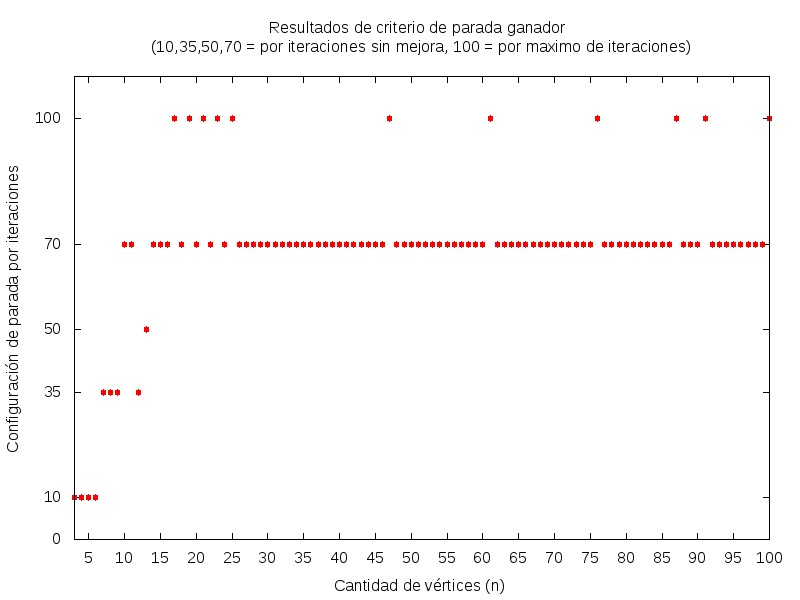
\includegraphics[width=\textwidth]{ejercicio-5-configuracion-conjunto-1.jpg}}
		\label{fig:ejercicio-5-configuracion-conjunto-1}
    \end{minipage}
\end{figure}
Podemos observar que para valores de $n$ menores a 15, muchas veces alcanza con 10, 35 ó 50 iteraciones sin mejora para ganar; es decir, en ningún caso usar las 100 iteraciones del otro criterio de parada mejora la solución, como preveíamos. Pero al aumentar el $n$, aunque claramente parar por 70 iteraciones sin mejora gana más veces, observamos que a veces resulta mejor el criterio de máximo de iteraciones, lo cual muestra falta de garantía de parar por iteraciones sin mejora.

Independientemente de qué criterio de parada sea mejor para cada $n$, veamos qué profundidad resultó ganadora. Veamos primero para cuantos $n$ resultó ganadora cada una:
\begin{figure}[H]
    \begin{minipage}[t]{\linewidth}
		\centering
		\frame{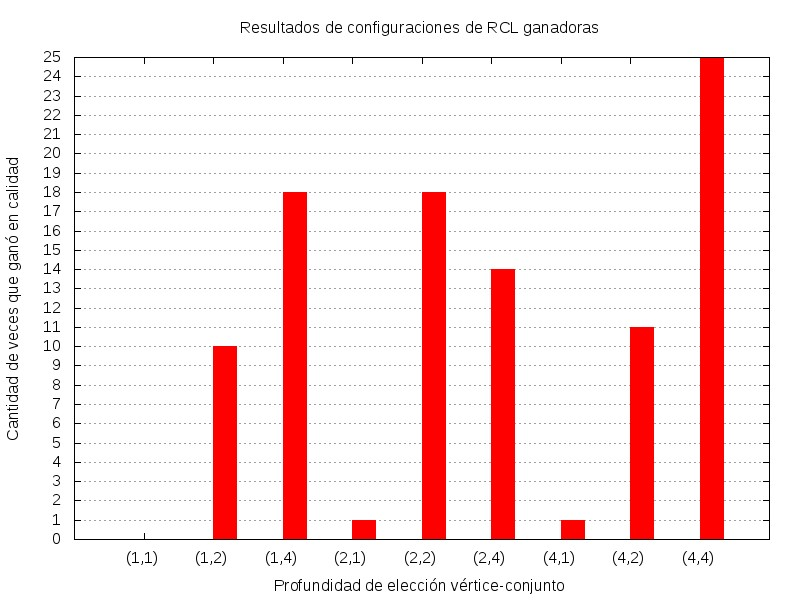
\includegraphics[width=\textwidth]{ejercicio-5-histograma-rcl-conjunto-1.jpg}}
		\label{fig:ejercicio-5-histograma-rcl-conjunto-1}
    \end{minipage}
\end{figure}
La primera observación es que usar de profundidad $(x,1)$ no es conveniente. En particular, $(1,1)$, que es equivalente a que la heurística golosa no tenga aleatoriedad, no resultó ganadora para ningún caso, como esperábamos. Usar $(4,4)$ gana más veces (25), y usar $(x,4)$ gana 57 veces, contra 39 ganadas de $(x,2)$. Fijando los conjuntos, $(1,x)$ gana 28 veces, $(2,x)$ gana 33, y $(4,x)$ gana 37 veces. Hasta ahora pareciera que $(4,4)$ es la mejor profundidad, pero tenemos que ver más detalladamente qué ocurre para cada $n$, porque si por ejemplo $(4,4)$ sólo ganara para las primeros 25 cantidades de nodos, pero fuera superada para $n \geq 27$, claramente sería una profundidad que no funciona para grafos con una cantidad elevada de nodos. Veamos entonces cuál profundidad gana para cada $n$:
\begin{figure}[H]
    \begin{minipage}[t]{\linewidth}
		\centering
		\frame{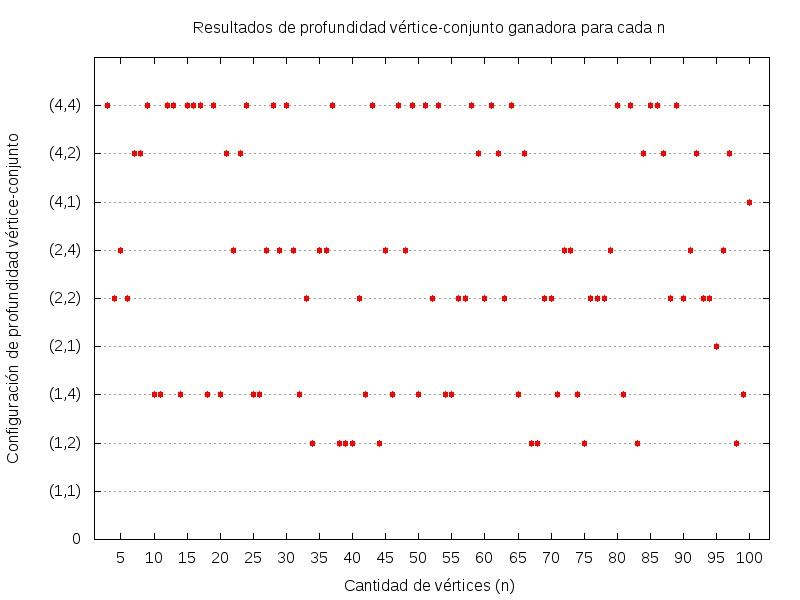
\includegraphics[width=\textwidth]{ejercicio-5-configuracion-profundidad-conjunto-1.jpg}}
		\label{fig:ejercicio-5-configuracion-profundidad-conjunto-1}
    \end{minipage}
\end{figure}
Podemos ver en el gráfico que $(4,4)$ gana de manera consistente, excepto para los $n$ más altos, para los cuales no parece haber claramente un ganador, ya que ganan casi todas las configuraciones. Hay un problema más: no sabemos exactamente por cuánto gana una profundidad. Vamos a usar el cálculo paralelo que hicimos, la suma de los pesos de cada configuración para las 10.000 instancias, para ver qué tan alejadas están verdaderamente las configuraciones de profundidad. Veamos los pesos acumulados de iteraciones sin mejora con valor 70 para cada profundidad $(x,y)$:
\begin{table}[H]
    \begin{center}
        \begin{tabular}{ | l | l | l | l |}
        \hline
        (x,y)   & 1                 & 2                 & 4 \\ \hline
        1       & 459037888         & 432225472         & 432218464 \\ \hline
        2       & 433368064         & 432117408         & 432198464 \\ \hline
        4       & 432523232         & 432218784         & 432113312 \\
        \hline
        \end{tabular}
        \caption{Peso acumulado para cada configuración}
    \end{center}
\end{table}
\begin{table}[H]
    \begin{center}
        \begin{tabular}{ | l | l | l | l |}
        \hline
        (x,y)   & 1                 & 2                 & 4 \\ \hline
        1       & 6.2309\%         & 0.0259\%         & 0.0243\% \\ \hline
        2       & 0.2903\%         & 0.0009\%         & 0.0197\% \\ \hline
        4       & 0.0948\%         & 0.0244\%         & 0.0000\% \\
        \hline
        \end{tabular}
        \caption{Error relativo de cada configuración contra el peso de la configuración $(4,4)$}
    \end{center}
\end{table}
$(4,4)$ logra el menor peso, y $(1,1)$ el peor (siendo $6.23\%$ más pesada). En particular, la primera columna, es decir, las profundidades $(x,1)$ son las tres peores. Pero el resto de las configuraciones no son mucho más pesadas que $(4,4)$ (la más pesada de éstas, $(1,2)$, sólo es un $0.026\%$ más pesada. En particular, $(2,2)$ es la más cercana siendo sólamente $0.0009479\%$ más pesada. Si tuviéramos que elegir entre fijar alguna profundidad en 1, y poder variar la otra, claramente podemos sacar como conclusión que aleatorizar la elección del conjunto es más importante que aleatorizar la elección del vértice a insertar. Aunque por otro lado, vemos que aumentar la profundidad de la elección de vértices también mejora las soluciones.

\noindent Por todo lo anterior, decidimos usar la configuración siguiente:
\begin{itemize}
    \item Criterio de parada: iteraciones sin mejora.
    \item Profundidad elección vértice-conjunto: $(4,4)$.
\end{itemize}

\subsubsection{Test de calidad}

En este test comparamos los pesos de las soluciones dadas por la GRASP con la configuración que elegimos (iteraciones sin mejora y profundidad $(4,4)$), contra los pesos de las soluciones óptimas obtenidas del algoritmo exacto. Lo hicimos hasta $n = 23$ por la complejidad temporal no polinomial del algoritmo exacto. 

Variamos el límite de iteraciones en potencias de 2: tomamos los valores $2^i$ con $i = \{0,1,...,9\}$. Para cada uno, calculamos el promedio de los errores relativos (en porcentaje) de las intancias de $n$ nodos, para $n = \{3,4,...,23\}$. Veamos los resultados:

\begin{figure}[H]
    \begin{minipage}[t]{\linewidth}
		\centering
		\frame{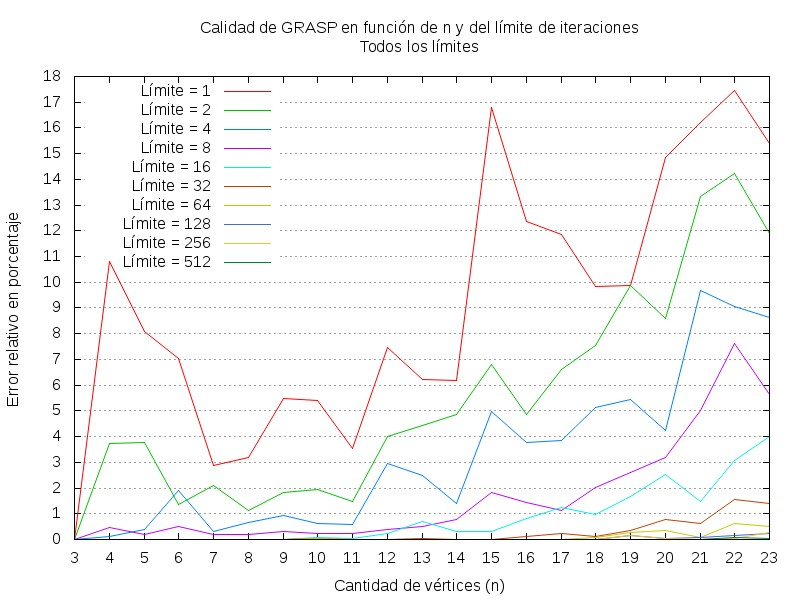
\includegraphics[width=\textwidth]{ejercicio-5-calidad-todos-conjunto-1.jpg}}
		\label{fig:ejercicio-5-calidad-todos-conjunto-1}
    \end{minipage}
\end{figure}

Como era de esperar, a mayor límite de iteraciones, mejor solución devuelve la GRASP. Tomar como límite una sola iteración tiene la peor performance, superando en el peor caso el $17\%$. Además, podemos ver que el error relativo para cualquier valor de iteraciones aumenta con el $n$, lo cual sugiere que no alcanza con fijar un cierto límite si no se sabe la máxima cantidad de vértices que van a tener los grafos de las instancias de entrada.

Veamos más en detalle lo que ocurre con los límites de iteraciones más altos, que dan los mejores resultados:

\begin{figure}[H]
    \begin{minipage}[t]{\linewidth}
		\centering
		\frame{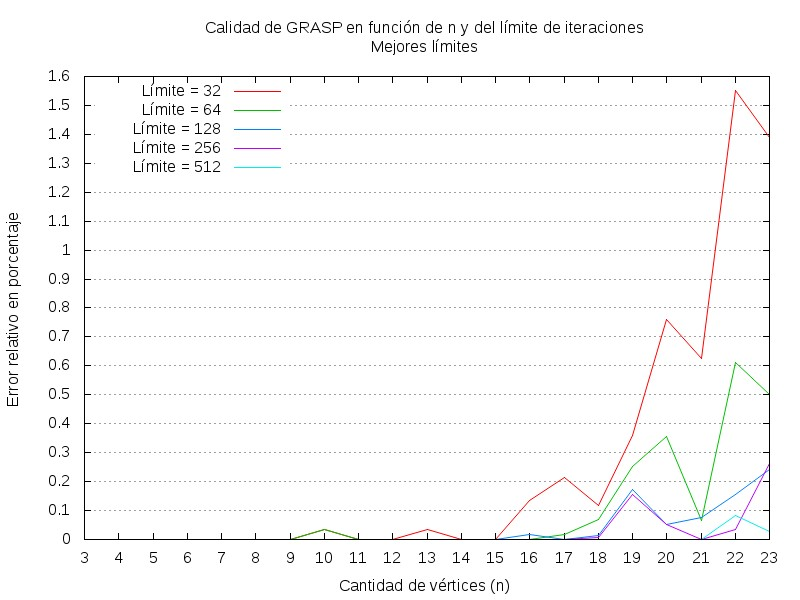
\includegraphics[width=\textwidth]{ejercicio-5-calidad-mejores-conjunto-1.jpg}}
		\label{fig:ejercicio-5-calidad-mejores-conjunto-1}
    \end{minipage}
\end{figure}

Nuevamente notamos que sigue valiendo la observación anterior para los mejores límites, esto es, tienden a crecer con $n$, incluso lo más altos. Solamente usar 512 iteraciones se mantiene por debajo del $0.1\%$, pero conjeturamos que al aumentar $n$, también crecerá y deberá usarse más de 512 iteraciones de límite para obtener una calidad menor a esa cota.

\subsubsection{Test de tiempo de ejecución}

Calculamos los promedios de los tiempos de ejecución para las instancias de cada $n$, con $n = \{3,4,...,100\}$. Lo hicimos para los dos criterios de parada que usamos en el test de configuración, es decir, usamos máximo de iteraciones con límite $100$, e iteraciones sin mejora con límite $70$; y para cada uno, usamos dos profundidades: $(2,2)$ y $(4,4)$. Con esto queremos ver si como supusimos, usar el criterio de iteraciones sin mejora efectivamente hace menos iteraciones para valores bajos $n$, y hace más para valores altos. Además queremos testear si aumentar la profundidad también aumenta los tiempos.

\begin{figure}[H]
    \begin{minipage}[t]{\linewidth}
		\centering
		\frame{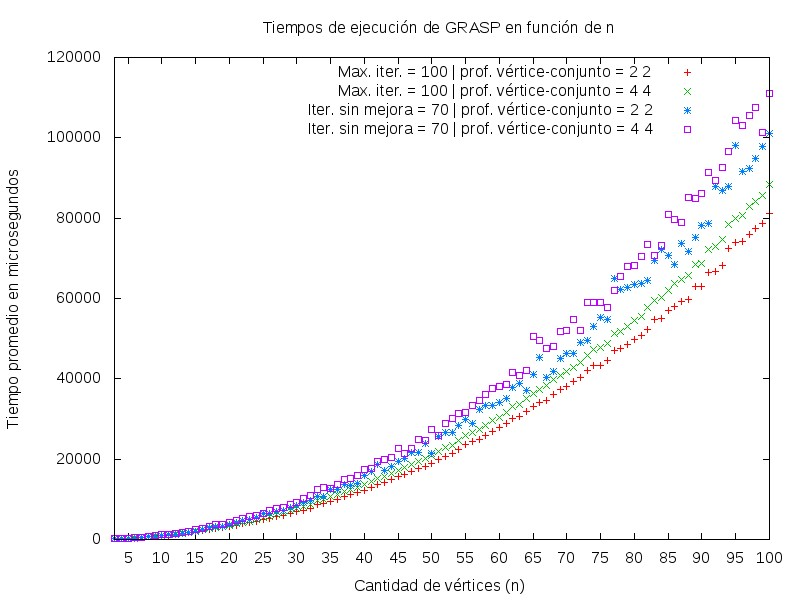
\includegraphics[width=\textwidth]{ejercicio-5-tiempos-grasp-conjunto-1.jpg}}
		\label{fig:ejercicio-5-tiempos-grasp-conjunto-1}
    \end{minipage}
\end{figure}

Vemos por un lado que a mayor $n$, el criterio de iteraciones sin mejora con ambas profundidades toma más tiempo que el criterio de iteraciones máximas, y que para cada una de ellas, usar más profundidad lleva también más tiempo. Lo primero lo explicamos con nuestra hipótesis: iteraciones sin mejora hace más iteraciones que el máximo a mayor $n$, y esta es una de las razones por las que termina dando mejores soluciones. Por otro lado, usar más profundidad hace que la golosa aleatorizada provea soluciones más distantes, y que haya más probabilidad de que la búsqueda local las mejore para superar a la mejor partición hasta el momento. Esto sugiere que usar más profundidad genera mejores soluciones. Falta ver qué ocurre para los primeros $n$:

\begin{figure}[H]
    \begin{minipage}[t]{\linewidth}
		\centering
		\frame{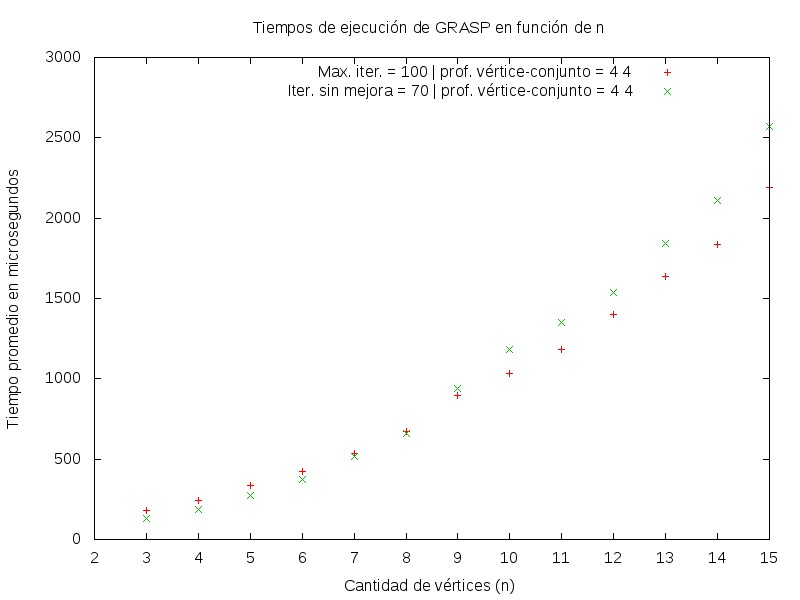
\includegraphics[width=\textwidth]{ejercicio-5-tiempos-grasp-primeros-nodos-conjunto-1.jpg}}
		\label{fig:ejercicio-5-tiempos-grasp-primeros-nodos-conjunto-1}
    \end{minipage}
\end{figure}

Como preveíamos, para grafos pequeños termina antes usar iteraciones sin mejora, aunque rápidamente iteraciones sin mejora comienza a superar las 100 iteraciones, y por esto es mayor para $n \geq 9$. La razón por la cual la diferencia es poco apreciable es que estamos usando como límite de iteraciones sin mejora a 70, pero ya vimos en el test de configuración que para valores menores a 15 podríamos usar 10, 35 ó 50 y así ---sin perder calidad--- obtener mayores diferencias en el tiempo de ejecución.
